\section{Modèle d'exécution fluxionnel}

\subsection{Fluxions}

Le modèle d'exécution fluxionnel à pour fonction de manipuler et d'invoquer des unités d'exécution autonomes n'ayant pour paramètre d'entrée et de sortie que des flux, c'est à dire des séquences continues et infinies de données agrégés par messages.
Nous avons appelé ce type d'unité d'exécution autonome une fluxion.
C'est à dire une fonction, au sens de la programmation fonctionnelle, dépendant exclusivement de flux de données.
Elle est composée d'un nom unique, d'une fonction de traitement, et d'un contexte mémoire au moment de son exécution.

Les entrées et sorties d'une fluxion sont des flux, c'est à dire une suite de messages.
% Un flux est un ensemble de messages à destination d'une fluxion.
Les messages sont composés du nom de la fluxion destinataire et d'un corps, et sont acheminés par un système de messagerie d'écrit dans la prochaine section.
Ils représentent à la fois le signal d'invocation, et les données nécessaires à cette invocation.
Après avoir traité un message, la fonction de traitement modifie son contexte local, puis termine son exécution en renvoyant un message sur son flux de sortie.
Chaque fluxion renvoie un message unique à destination d'une ou plusieurs fluxions.
Le contexte d'exécution de la fonction de traitement est composé de l'ensemble des variables de mémoire dont dépend la fluxion pour poursuivre un traitement entre deux exécutions.

Les fluxions forment des chaînes de traitement liés par les flux.
L'ensemble de ces chaînes de traitement forme un graphe direct orienté.

\subsection{Système de messagerie}

Le système de messagerie est le cœur du modèle d'exécution fluxionnel.
Il a pour fonction, à la fois d'acheminer les flux de messages entres les fluxions, et d'invoquer les fluxions.

Il est construit autour d'une file de messages.
Ceux-ci sont traités les uns après les autres par l'invocation de la fluxion destination.
L'utilisation d'une file de messages permet d'exécuter plusieurs chaîne de traitement en parallèle de manière équitable, et de ne pas faire de différence dans l'ordonnancement entre les messages locaux et les messages provenant du réseau.
Le cycle de vie du système de messagerie est illustré dans la figure \ref{fig:messagerie}.

\begin{figure}[h!]
  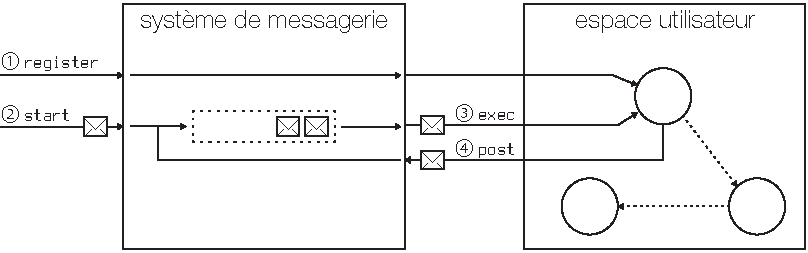
\includegraphics[width=0.5\textwidth]{schema-message.pdf}
  \caption{Schema du système de messagerie}
  \label{fig:messagerie}
\end{figure}

Chaque fluxion dois être enregistré dans le système de messagerie.
Cet enregistrement associe une fonction de traitement à un nom, et un contexte d'exécution propre.
Le système de messagerie achemine les flux de messages en se basant sur les noms des fluxions.
C'est pourquoi il ne peut pas exister plusieurs fluxions ayant le même nom.
Lors de cet enregistrement, il est possible d'initialiser le contexte d'exécution.
L'enregistrement se fait à l'aide de la fonction \texttt{register(<nom>, <fn>, <contexte>)}, étape \circled{1} sur la figure \ref{fig:messagerie}.
Une fluxion peut elle-même enregistrer d'autres fluxions dynamiquement.

Pour déclencher une chaîne de fluxions un premier message est envoyé à destination d'une fluxion par l'intermédiaire du système de messagerie, en utilisant la fonction \texttt{start(<msg>)}, étape \circled{2} sur le figure \ref{fig:messagerie}.
Cette fonction va placer un premier message dans la file.
Le système exécute la fonction de traitement destinataire de ce premier message, étape \circled{3} sur le figure \ref{fig:messagerie}.
Le message résultat de cette exécution est alors empilé dans la file de message, étape \circled{4} sur le figure \ref{fig:messagerie}.

L'algorithme \ref{alg:traitement} formalise précisément le comportement du système de messagerie lors de l'appel de la fonction \texttt{start}s.
Tandis que l'algorithme \ref{alg:parcours} explique le parcours de la file de messages.

\begin{algorithm}
\caption{Algorithme de traitement de la file de messages}
\label{alg:traitement}
\begin{algorithmic}
\Function{processMsg}{$msg$}
\For{$dest$ \textbf{in} $msg.dest$}
\State $fluxion \gets lookup(dest)$
\State $message \gets$ \Call{exec}{$fluxion, msg.body$} \Comment{étape \circled{3}}
\State \Call{enqueue}{$message$} \Comment{étape \circled{4}}
\EndFor
\EndFunction
\end{algorithmic}
\end{algorithm}

\begin{algorithm}
\caption{Algorithme de parcours de la file}
\label{alg:parcours}
\begin{algorithmic}
\While{$true$}
\While{$msg$ \textbf{presents in} $msgQueue$}
\State $msg \gets$ \Call{dequeue}{\null}
\State \Call{ProcessMsg}{$msg$}
\EndWhile
\EndWhile
\end{algorithmic}
\end{algorithm}

\subsection{Interfaces externes}

Les fluxions ne peuvent échanger qu'aux autres fluxions à l'intérieur du modèle d'exécution.
Afin de pouvoir interagir avec le monde extérieur, il faut définir des interfaces de bordure entre l'intérieur et l'extérieur du système. Ces bordures sont capable à la fois d'interagir avec le système et avec l'extérieur.
Ce lien d'interaction avec l'extérieur compromet leur autonomie.


Notre approche repose sur une espérance de gain technologique principalement sur les architectures Web.
L'interface d'entré visé est l'intégration des interfaces REST, mais tout autre point d'entrée est valable tant qu'une interface de bordure en flux peut être défini.

Dans notre approche, il existe deux types d'interface de bordures pour le Web :

\begin{itemize}
	\item[les \textbf{entrées}]
    permettent de recevoir des connections clientes entrantes suivant le protocole HTTP.
    C'est donc le premier maillon de la chaîne de traitement.
    Pour chaque connexion entrante, l'entrée va générer une fluxion de sortie permettant de répondre au client.
	\item[les \textbf{sorties}]
    permettent d'envoyer le résultat de la chaîne de traitement au client.
    C'est donc le dernier maillon de la chaîne de traitement.
\end{itemize}


Le schéma \ref{fig:schemaweb} présente les éléments d'un système Web fluxionnel et détaille les étapes d'acheminement d'un message par le système de messagerie.

\begin{figure}[h!]
	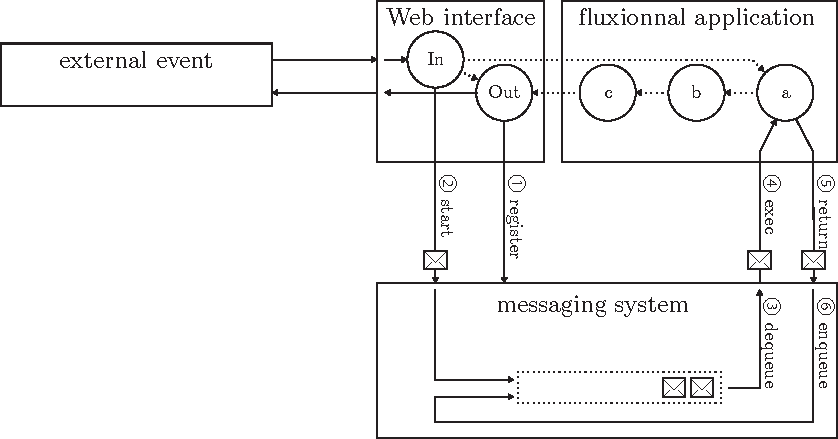
\includegraphics[width=0.5\textwidth]{schema-web.pdf}
	\caption{Schema d'un système fluxionnel avec une interface web}
	\label{fig:schemaweb}
\end{figure}

Le système Web est donc le déclencheur d'une chaîne de traitement de requêtes.
À chaque nouvelle requête d'un utilisateur, la fonction \texttt{start(<query>)} du système de messagerie est appelée.
Au démarrage du système Web, deux fluxions de bordure sont lancées.
La bordure entrante n'est pas enregistré dans le système de messagerie.
Elle prend les paramètres de la requête Web, place l'identifiant de la connexion client dans le contexte de la demi-fluxion de sortie, puis lance le traitement de la requête en invoquant la fonction \texttt{start} du système de messagerie.

\subsection{Exemple de fluxion}

Afin d'illustrer le modèle d'exécution fluxionnel, nous présentons ici un exemple de son utilisation à travers un simple service de comptage de visite.

Ce service permet de compter le nombre de connexions HTTP de chaque utilisateur sur ce service et renvoie ce nombre dans la réponse.

L'extrait de code \ref{lst:classique} représente ce service de comptage exprimé dans un modèle classique.

\begin{figure}
  \begin{code}
  var app = require('express')();

  var count = {};

  app.get('/:id', function(req, res){
    res.send(req.params.id + '[' + (count[req.params.id] = (count[req.params.id] + 1) || 1 ) + ']');
  });

  port = 8080;
  app.listen(port);
  console.log("Listening port: "+port);
  \end{code}
  \caption{Code classique}
  \label{lst:classique}
\end{figure}

L'extrait de code \ref{lst:fluxionnel} représente ce même service de comptage dans le modèle fluxionnel.

\begin{figure}
  \begin{code}
  var flx = require('./lib/flx')
    , express = require('express')
    , app = express();

  // 1
  app.get('/:id', function(req, res) {
    var uid = req.params.id;
    var cid = req.client._idleStart;

    flx.start(flx.m("output", {cid: cid, res: res}));
    flx.start(flx.m("input", {uid: uid, cid: cid}));
  })

  // 2
  flx.register("input", function(msg){
    this.uid[msg.uid] = this.uid[msg.uid] + 1 || 1;
    msg.count = this.uid[msg.uid];
    return this.m("view", msg);
  },{
    uid: {}
  });

  // 3
  flx.register("view", function(msg) {
    msg.view = msg.uid + "[" + msg.count + "]";
    msg.uid = undefined;
    msg.count = undefined;
    return this.m("output", msg);
  })

  // 4
  flx.register("output", function(msg){
    if (msg.res) {
      this.cid[msg.cid] = msg.res;
    } else {
      this.cid[msg.cid].send(msg.view.toString());
    }
    return undefined;
  }, {
    cid: {}
  })

  app.listen(8080);
  \end{code}
  \caption{Code fluxionnel}
  \label{lst:fluxionnel}
\end{figure}

La code classique est bien plus concis que le code fluxionnel du fait de la segmentation et de l'encapsulation impliqué par le modèle fluxionnel.

Le service à été ségmenté comme suit :
\begin{itemize}
  \item[\circled{1}] Le point d'entrée \texttt{app.get} réagit à la connexion d'un client et démarre la chaîne de traitement en appelant \texttt{start}.
  Ce n'est pas une fluxion, il n'est pas enregistré dans le système de messagerie, et est lié à la machine recevant les connections entrantes.
  \item[\circled{4}] Le point de sortie \texttt{output} est enregistré dans le système comme une fluxion mais elle est liée à la machine recevant les connexions clientes afin de pouvoir y répondre.
  \item[\circled{2}] La fluxion \texttt{input} est la première à recevoir le message indiquant une connexion cliente. Son traitement consiste à incrémenter le compteur de l'utilisateur présent dans son scope, et à renseigner ce compteur dans le message, avant de le renvoyer à la fluxion suivante.
  Elle contient l'ensemble de la logique de ce simple service. Pour des services réels, on trouverais à sa place l'ensemble des fluxions contenant la logique du service organisé en une ou plusieurs chaîne de traitement.
  \item[\circled{3}] La fluxion \texttt{view} récupère le message, et met en forme la réponse que recevra l'utilisateur, et l'envoie à la fluxion de sortie.
\end{itemize}

Ce service manipule principalement deux informations sur lesquelles qu'il est important de détailler.
D'une part, les connections clientes sont partagé entre l'entrée et la sortie.
Pour chaque connexion, l'entrée passe directement à la sortie un couple <id, res>.
id représente simplement un identifiant permettant de retrouver res, il est envoyé à la fluxion input.
res est la structure permettant de répondre au client.
Ce mécanisme provoque un échange important de donnée entre le point d'entrée et le point de sortie, et implique de passer l'identifiant sur toute la chaîne de traitement, jusqu'à sa réception au point de sortie.

Les messages échangés contiennent principalement deux informations importantes : les identifiants d'utilisateurs, permettant d'incrémenter un compteur pour chaque utilisateur, et les identifiants de connexion, permettant de lier une suite de messages avec la structure contenant la connexion HTTP.
Le point d'entrée, et le point de sortie du système doivent rester sur la machine où la connexion a eu lieu pour avoir accès à l'interface réseau, tandis que les autre fluxions n'ont pas cette obligation, et peuvent être migré.


Cet identifiant de connexion est nécessaire au point de sortie pour associer le résultat reçu avec la connexion vers laquelle le renvoyer à l'utilisateur.
Nous passons cet identifiant pour ne pas alourdir les échanges de messages avec la structure contenant la connexion HTTP.

Ainsi, la fluxion de sortie reçois des messages provenant de deux fluxions : le point d'entrée




